%%%%%%%%%%%%%%%%%%%%%%%%%%%%%%%%%%%%%%%%%
% University/School Laboratory Report
% LaTeX Template
% Version 3.1 (25/3/14)
%
% This template has been downloaded from:
% http://www.LaTeXTemplates.com
%
% Original author:
% Linux and Unix Users Group at Virginia Tech Wiki 
% (https://vtluug.org/wiki/Example_LaTeX_chem_lab_report)
%
% License:
% CC BY-NC-SA 3.0 (http://creativecommons.org/licenses/by-nc-sa/3.0/)
%
%%%%%%%%%%%%%%%%%%%%%%%%%%%%%%%%%%%%%%%%%

%----------------------------------------------------------------------------------------
%	PACKAGES AND DOCUMENT CONFIGURATIONS
%----------------------------------------------------------------------------------------

\documentclass{article}

%\usepackage[version=3]{mhchem} % Package for chemical equation typesetting
%\usepackage{siunitx} % Provides the \SI{}{} and \si{} command for typesetting SI units
\usepackage{graphicx} % Required for the inclusion of images
\usepackage{natbib} % Required to change bibliography style to APA
\usepackage{amsmath} % Required for some math elements 
\usepackage{listings}
\lstset{basicstyle=\small\ttfamily, breaklines=true}
\setlength\parindent{2pt} % Removes all indentation from paragraphs
\linespread{1.8}
%\renewcommand{\labelenumi}{\alph{enumi}.} % Make numbering in the enumerate environment by letter rather than number (e.g. section 6)

%\usepackage{times} % Uncomment to use the Times New Roman font

%----------------------------------------------------------------------------------------
%	DOCUMENT INFORMATION
%----------------------------------------------------------------------------------------

\title{Laboratory on Linux Kernel Haking\\ OS - Operating System} % Title

\author{Simone \textsc{Rossi}} % Author name

\date{\today} % Date for the report

\begin{document}

\maketitle % Insert the title, author and date

\begin{center}
\begin{tabular}{l r}
Date Performed: & \today \\ % Date the experiment was performed
Partners: & Simone Rossi \\ % Partner names
%& Mary Smith \\
%Instructor: & Professor Smith % Instructor/supervisor
\end{tabular}
\end{center}

% If you wish to include an abstract, uncomment the lines below
% \begin{abstract}
% Abstract text
% \end{abstract}

%----------------------------------------------------------------------------------------
%	SECTION 1
%----------------------------------------------------------------------------------------

\section{Compiling the Linux kernel}
To analyze thet version of the kernel currently under execution, the command to be typed is 
\texttt{uname -vr}\footnote{The command returns both the kernel version and release}.\\

From the source code of \texttt{linux-2.4}, I tried to remove the support for the Ext3 
filesystem. The new kernel has been compiled (computing all the dependencies and compiling
all the sources) and mount using \texttt{lilo}.\\

Of course now, without the support for this version of filesystem, the kernel could not correctly 
load and mount the root filesystem; as conseguence, it entered in the kernel panic state (with error
19) with no possibilities to be recovered.\\

\begin{figure}
\centering
  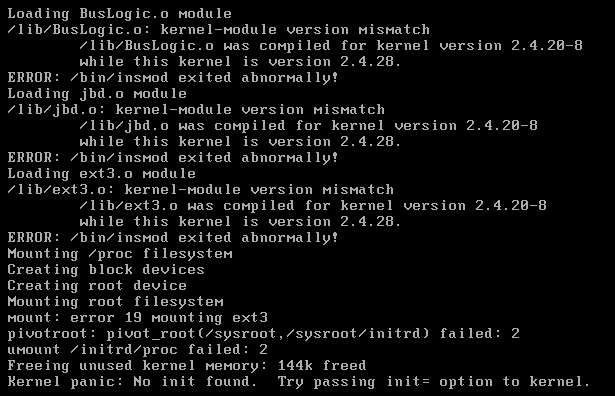
\includegraphics[width=\textwidth]{./kernel_panic.png}
\end{figure}


\section{Adding new system calls to Linux}
The man page of Linux describes the system call as a fundamental interface between an application and
the Linux kernel itself. [\dots] Usually they are not invoked directly but rather via wrapper functions.

The system calls deal with low aspects of the operating systems, while providing high-level Application
Programming Interface (API). 

\begin{figure}
\centering
  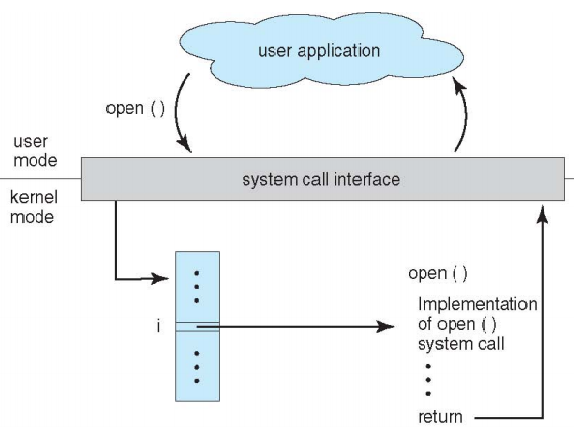
\includegraphics[width=\textwidth]{./syscall.png}
\end{figure}

Let's assume the user application calls a library function which actually during its execution makes a
system call to the kernel. The name of the system call is used as offset in a system call table and 
an interrupt is raised.\\ 

As explained in the document, to add new system calls to the kernel, two files should be modified
in order to let the system know the presence of new syscalls during the compilation:
\begin{itemize}
    \item \texttt{include/asm-i386/unistd.h} contains the system call numbers for the system call table
      and seven different "template" prototype for the function (with different numbers of parameters).
      \begin{figure}
      \centering
        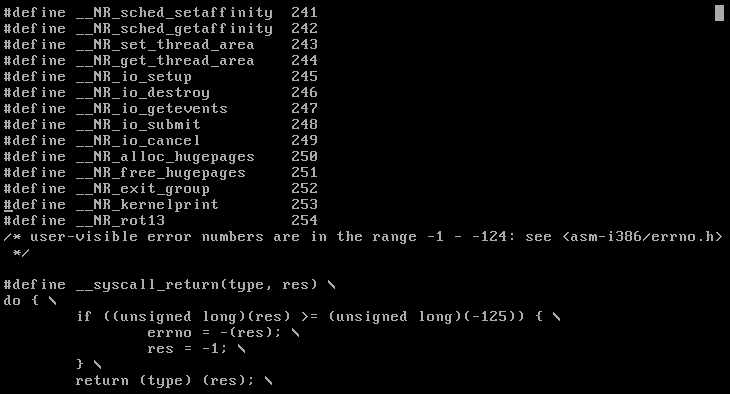
\includegraphics[width=.8\textwidth]{./unistd.png}
      \end{figure}
    \item \texttt{arch/i386/kernel/entry.S} contains the system call low level handling routines and 
      the ling between a system call and a entry of the systel call table.
      \begin{figure}
      \centering
        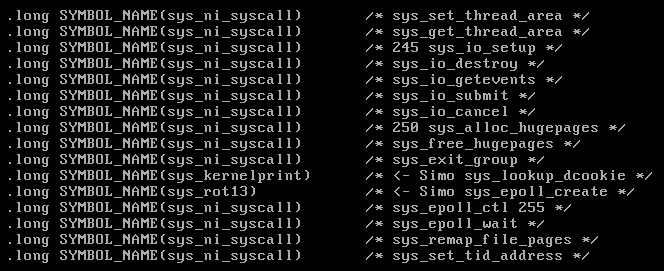
\includegraphics[width=.8\textwidth]{./entrys.png}
      \end{figure}
\end{itemize}


\end{document}
